\documentclass[10pt]{article}
\usepackage{tikz}
\usetikzlibrary{shapes.misc}
\usepackage[margin=0cm]{geometry}
\pagestyle{empty}
\tikzstyle{every node}=[cross out, draw, red]

\begin{document}

\vspace*{\fill}
\begin{center}
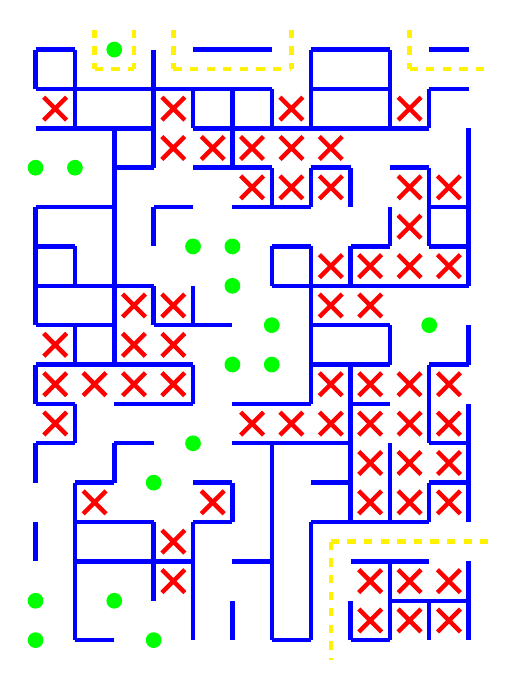
\begin{tikzpicture}[x=0.5cm, y=-0.5cm, ultra thick, blue]
% Walls
    \draw (0,0) -- (1,0);
    \draw (4,0) -- (6,0);
    \draw (7,0) -- (9,0);
    \draw (10,0) -- (11,0);
    \draw (0,1) -- (6,1);
    \draw (7,1) -- (9,1);
    \draw (10,1) -- (11,1);
    \draw (0,2) -- (3,2);
    \draw (4,2) -- (10,2);
    \draw (2,3) -- (3,3);
    \draw (4,3) -- (6,3);
    \draw (7,3) -- (8,3);
    \draw (9,3) -- (10,3);
    \draw (0,4) -- (2,4);
    \draw (3,4) -- (4,4);
    \draw (5,4) -- (7,4);
    \draw (10,4) -- (11,4);
    \draw (0,5) -- (1,5);
    \draw (6,5) -- (7,5);
    \draw (8,5) -- (9,5);
    \draw (10,5) -- (11,5);
    \draw (0,6) -- (3,6);
    \draw (6,6) -- (11,6);
    \draw (0,7) -- (2,7);
    \draw (3,7) -- (5,7);
    \draw (7,7) -- (9,7);
    \draw (0,8) -- (4,8);
    \draw (7,8) -- (9,8);
    \draw (10,8) -- (11,8);
    \draw (0,9) -- (1,9);
    \draw (2,9) -- (4,9);
    \draw (5,9) -- (7,9);
    \draw (8,9) -- (9,9);
    \draw (0,10) -- (1,10);
    \draw (2,10) -- (3,10);
    \draw (5,10) -- (8,10);
    \draw (10,10) -- (11,10);
    \draw (1,11) -- (2,11);
    \draw (4,11) -- (5,11);
    \draw (7,11) -- (8,11);
    \draw (10,11) -- (11,11);
    \draw (1,12) -- (3,12);
    \draw (4,12) -- (5,12);
    \draw (7,12) -- (10,12);
    \draw (1,13) -- (4,13);
    \draw (5,13) -- (6,13);
    \draw (8,13) -- (10,13);
    \draw (9,14) -- (11,14);
    \draw (1,15) -- (2,15);
    \draw (6,15) -- (7,15);
    \draw (8,15) -- (9,15);
    \draw (0,0) -- (0,1);
    \draw (0,4) -- (0,7);
    \draw (0,8) -- (0,9);
    \draw (0,10) -- (0,11);
    \draw (0,12) -- (0,13);
    \draw (1,0) -- (1,2);
    \draw (1,5) -- (1,6);
    \draw (1,7) -- (1,8);
    \draw (1,9) -- (1,10);
    \draw (1,11) -- (1,15);
    \draw (2,2) -- (2,8);
    \draw (2,10) -- (2,11);
    \draw (3,0) -- (3,3);
    \draw (3,4) -- (3,5);
    \draw (3,6) -- (3,7);
    \draw (3,12) -- (3,14);
    \draw (4,1) -- (4,2);
    \draw (4,6) -- (4,7);
    \draw (4,8) -- (4,9);
    \draw (4,12) -- (4,15);
    \draw (5,1) -- (5,3);
    \draw (5,11) -- (5,12);
    \draw (5,14) -- (5,15);
    \draw (6,1) -- (6,2);
    \draw (6,3) -- (6,4);
    \draw (6,5) -- (6,6);
    \draw (6,10) -- (6,15);
    \draw (7,0) -- (7,2);
    \draw (7,3) -- (7,4);
    \draw (7,5) -- (7,9);
    \draw (7,12) -- (7,15);
    \draw (8,3) -- (8,4);
    \draw (8,5) -- (8,6);
    \draw (8,8) -- (8,12);
    \draw (8,14) -- (8,15);
    \draw (9,0) -- (9,2);
    \draw (9,4) -- (9,5);
    \draw (9,7) -- (9,8);
    \draw (9,10) -- (9,12);
    \draw (9,13) -- (9,15);
    \draw (10,1) -- (10,2);
    \draw (10,3) -- (10,5);
    \draw (10,8) -- (10,10);
    \draw (10,11) -- (10,12);
    \draw (10,14) -- (10,15);
    \draw (11,2) -- (11,6);
    \draw (11,7) -- (11,8);
    \draw (11,9) -- (11,12);
    \draw (11,13) -- (11,15);
% Pillars
    \fill[green] (2,0) circle(0.2);
    \fill[green] (0,3) circle(0.2);
    \fill[green] (1,3) circle(0.2);
    \fill[green] (4,5) circle(0.2);
    \fill[green] (5,5) circle(0.2);
    \fill[green] (5,6) circle(0.2);
    \fill[green] (6,7) circle(0.2);
    \fill[green] (10,7) circle(0.2);
    \fill[green] (5,8) circle(0.2);
    \fill[green] (6,8) circle(0.2);
    \fill[green] (4,10) circle(0.2);
    \fill[green] (3,11) circle(0.2);
    \fill[green] (0,14) circle(0.2);
    \fill[green] (2,14) circle(0.2);
    \fill[green] (0,15) circle(0.2);
    \fill[green] (3,15) circle(0.2);
% Inner points in accessible cul-de-sacs
    \node at (0.5,1.5) {};
    \node at (3.5,1.5) {};
    \node at (6.5,1.5) {};
    \node at (9.5,1.5) {};
    \node at (3.5,2.5) {};
    \node at (4.5,2.5) {};
    \node at (5.5,2.5) {};
    \node at (6.5,2.5) {};
    \node at (7.5,2.5) {};
    \node at (5.5,3.5) {};
    \node at (6.5,3.5) {};
    \node at (7.5,3.5) {};
    \node at (9.5,3.5) {};
    \node at (10.5,3.5) {};
    \node at (9.5,4.5) {};
    \node at (7.5,5.5) {};
    \node at (8.5,5.5) {};
    \node at (9.5,5.5) {};
    \node at (10.5,5.5) {};
    \node at (2.5,6.5) {};
    \node at (3.5,6.5) {};
    \node at (7.5,6.5) {};
    \node at (8.5,6.5) {};
    \node at (0.5,7.5) {};
    \node at (2.5,7.5) {};
    \node at (3.5,7.5) {};
    \node at (0.5,8.5) {};
    \node at (1.5,8.5) {};
    \node at (2.5,8.5) {};
    \node at (3.5,8.5) {};
    \node at (7.5,8.5) {};
    \node at (8.5,8.5) {};
    \node at (9.5,8.5) {};
    \node at (10.5,8.5) {};
    \node at (0.5,9.5) {};
    \node at (5.5,9.5) {};
    \node at (6.5,9.5) {};
    \node at (7.5,9.5) {};
    \node at (8.5,9.5) {};
    \node at (9.5,9.5) {};
    \node at (10.5,9.5) {};
    \node at (8.5,10.5) {};
    \node at (9.5,10.5) {};
    \node at (10.5,10.5) {};
    \node at (1.5,11.5) {};
    \node at (4.5,11.5) {};
    \node at (8.5,11.5) {};
    \node at (9.5,11.5) {};
    \node at (10.5,11.5) {};
    \node at (3.5,12.5) {};
    \node at (3.5,13.5) {};
    \node at (8.5,13.5) {};
    \node at (9.5,13.5) {};
    \node at (10.5,13.5) {};
    \node at (8.5,14.5) {};
    \node at (9.5,14.5) {};
    \node at (10.5,14.5) {};
% Entry-exit paths without intersections
    \draw[dashed, yellow] (1.5,0.5) -- (2.5,0.5);
    \draw[dashed, yellow] (3.5,0.5) -- (6.5,0.5);
    \draw[dashed, yellow] (9.5,0.5) -- (11.5,0.5);
    \draw[dashed, yellow] (7.5,12.5) -- (11.5,12.5);
    \draw[dashed, yellow] (1.5,-0.5) -- (1.5,0.5);
    \draw[dashed, yellow] (2.5,-0.5) -- (2.5,0.5);
    \draw[dashed, yellow] (3.5,-0.5) -- (3.5,0.5);
    \draw[dashed, yellow] (6.5,-0.5) -- (6.5,0.5);
    \draw[dashed, yellow] (7.5,12.5) -- (7.5,15.5);
    \draw[dashed, yellow] (9.5,-0.5) -- (9.5,0.5);
\end{tikzpicture}
\end{center}
\vspace*{\fill}

\end{document}
